%% ============ SECTION 2 ============ %%
\newpage
\section{ Problem 2.}
\textit{
  Find the maximum and minimum values of $ z = 2x^2 - 2xy + y^3 $ subject to the single constraint $ x^2 + y^2 = 4 $.
  \begin{enumerate}[label=(\alph*)]
    \item Using Lagrange multiplier method.
    \item Using contour plot (Draw the contour plot of the function and
    the constraint curve in the same figure).  
  \end{enumerate}
}

\vspace*{1cm}

\textbf{Theory: }

To find the maximum and minimum value of $f(x,y) = 2x^2 - 2xy + y^3$ subject to the single constraint $ g(x,y) = x^2 + y^2 = 4 $, we need to use the Lagrange multiplier method.\\

Lagrange multiplier method is a technique for finding maximum or minimum values of some multivariable function $f(x,y,z, ...)$ subject to a constraint of the form $g(x,y,z,...)$.\\

For example, a function of 2 variables can be used to explain the method. We get started by finding the extreme values of $f(x,y)$ subject to a constraint $g(x,y)$. In other words, we find the points satisfying the condition that points $(x,y)$ lie on the level curve $g(x,y)=k$.  The figure below shows this curve together with several level curves of $f(x,y)$. These have the equations $f(x,y) = c$  where  $c \in \{7,8,9,10,11\}$.

\begin{figure}[H]
  \centering
  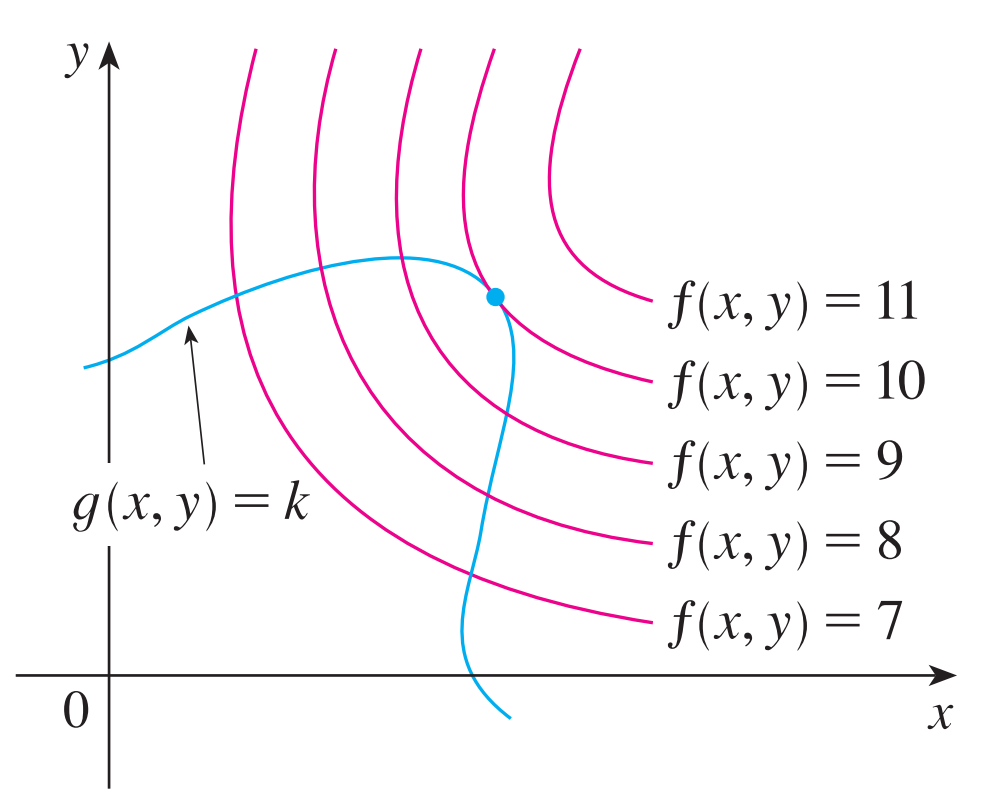
\includegraphics[width=9cm]{graphics/2a.png}
  % \caption{}
\end{figure}

The graph illustrates that the maximum value occupied at the point where $f(x,y)=10$ intersecting $g(x,y)=k$. Analyzing the graph, we can easily see the fact that the maximum value appears when those 2 functions touch each other and they have the same tangent line. Thus the normal lines at the point of intersection $(x_0,y_0)$ are identical. So the gradient vectors are parallel; Therefore, $\nabla f(x_0,y_0) = \lambda g(x_0,y_0)$ where $\lambda$ is a scalar. \\[6pt]
For some scalar $\lambda$. The scalar parameter is called a Lagrange multiplier. The procedure based on the above equation is as follows. We have from the chain rule,
$$ \dfrac{df(x, y)}{dxdy} = \dfrac{\partial f(x, y)}{\partial x} dx + \dfrac{\partial f(x, y)}{\partial y} = 0,\quad \dfrac{dg(x, y)}{dxdy} = \dfrac{\partial g(x, y)}{\partial x} dx + \dfrac{\partial g(x, y)}{\partial y} $$ \\[6pt]
Multiplying the second equation by $\lambda$ and then add to first equation yield:
$$ \left( \dfrac{\partial f(x, y)}{\partial x} + \dfrac{\partial g(x, y)}{\partial x} \right)dx + \left( \dfrac{\partial f(x, y)}{\partial y} + \dfrac{\partial g(x, y)}{\partial y} \right)dy = 0 $$\\[6pt]
Then we can rewrite the expression as the vector equation:
$$ \nabla f(x_0, y_0) =\lambda \nabla g(x_0, y_0) $$
Thus, the maximum and minimum values of $f(x,y)$ subject to the constraint $g(x_0,y_0)=0$  can be found by solving the following set of equations.
$$ \dfrac{\partial f(x, y)}{\partial x} + \dfrac{\partial g(x, y)}{\partial x} = 0 $$
$$ \dfrac{\partial f(x, y)}{\partial y} + \dfrac{\partial g(x, y)}{\partial y} = 0 $$
$$ g(x, y) = 0 $$\\[6pt]
The Lagrange multiplier method allows us to find the values of the variables that optimize the objective function subject to the given constraints. This technique is widely used in various fields of mathematics, physics, and engineering, particularly in optimization problems involving constraints.\\[6pt]

\textbf{Solving Problem using Lagrange multiplier method:}\\[6pt]
$$ Let \quad  f(x,y)= z = 2x^2-2xy+y^3 \quad and \quad g(x,y)=x^2 + y^2- 4 $$
Therefore, we obtain a system of equations:
\[
\begin{cases}
  x - 2y + 2 \lambda x &= 0 \qquad (1) \\
  2x + 3y^2 + 2 \lambda x &= 0 \qquad (2) \\
  x^2 + y^2 - 4 &= 0 \qquad (3) \\
\end{cases}
\]

Solve the equation $(1)$ for $x$, we get:
$$ x = \dfrac{y}{2 + \lambda} $$

Substitute $x$ in the equation $(2)$:
$$ 3y^2 + 2 \lambda y - \dfrac{2y}{2 + \lambda} = 0 \quad (4)$$

Then we substitute $x$ into the equation $(3)$ and solve for $y$:
\begin{align*}
  \dfrac{y^2}{(2 + \lambda)^2} + y^2 &= 4 \\
  y^2 &= \dfrac{4}{1 + \dfrac{1}{(2 + \lambda)^2}} \\
  y &= \pm \dfrac{2}{  \sqrt{1 + \dfrac{1}{(2+ \lambda)^2}}  } \\
\end{align*}

Plug $y = -\dfrac{2}{  \sqrt{1 + \dfrac{1}{(2+ \lambda)^2}}  }$ to equation $(4)$ then we obtain:
$$ 3 \dfrac{4}{1 + \dfrac{1}{(2+x)^2}} + 2 \lambda \dfrac{-2}{ \sqrt{1 + \dfrac{1}{(2 + \lambda)^2}} } - \dfrac{-4}{(2 + \lambda) \sqrt{1 + \left(\frac{1}{2 + \lambda}\right)^2} } = 0 $$\\[6pt]

Then we obtain 2 values of $\lambda$:
$$ \lambda = 3.13935 \quad and \quad \lambda = -2.31197 $$

With $y = \dfrac{2}{  \sqrt{1 + \dfrac{1}{(2+ \lambda)^2}}  }$ we have another equation:
$$ 3 \dfrac{4}{1 + \dfrac{1}{(2+x)^2}} + 2 \lambda \dfrac{2}{ \sqrt{1 + \dfrac{1}{(2 + \lambda)^2}} } - \dfrac{4}{(2 + \lambda) \sqrt{1 + \left(\frac{1}{2 + \lambda}\right)^2} } = 0 $$\\[6pt]

Also, two other values of $\lambda$:
$$ \lambda = -1,03873 \quad and \quad \lambda = -3.1317 $$

Last step is to compute value of $x$ and $y$ according to each value of $\lambda$: \\
With $\lambda = 3.13935$:
$$ y = -\dfrac{2}{ \sqrt{1 + \dfrac{1}{(2 + \lambda)^2}} } = -\dfrac{2}{ \sqrt{1 + \dfrac{1}{(2 + 3.13935)^2}} } = -1.96318$$
$$ x = \dfrac{y}{2 + \lambda} = \dfrac{-1.96318}{2 + 3.13935} = -0.38199 $$

With $\lambda = -2.31197$: 
$$ y = -\dfrac{2}{ \sqrt{1 + \dfrac{1}{(2 + \lambda)^2}} } = -\dfrac{2}{ \sqrt{1 + \dfrac{1}{(2 -2.31197)^2}} } = -0.595631$$
$$ x = \dfrac{y}{2 + \lambda} = \dfrac{-0.595631}{2 -2.31197} = 1.90925 $$

With $\lambda = -1,03873$: 
$$ y = -\dfrac{2}{ \sqrt{1 + \dfrac{1}{(2 + \lambda)^2}} } = -\dfrac{2}{ \sqrt{1 + \dfrac{1}{(2 -1,03873)^2}} } =1.38602$$
$$ x = \dfrac{y}{2 + \lambda} = \dfrac{1.38602}{2 -1,03873} = 1.44186 $$

With $\lambda =-3.13172$: 
$$ y = -\dfrac{2}{ \sqrt{1 + \dfrac{1}{(2 + \lambda)^2}} } = -\dfrac{2}{ \sqrt{1 + \dfrac{1}{(2 -3.13172)^2}} } = 1.49874$$
$$ x = \dfrac{y}{2 + \lambda} = \dfrac{1.49874}{2 -3.13172} = -1.3243 $$\\[6pt]

After obtaining all value of $x, y$ in each case of $\lambda$, we evaluate $f$ at all the point $(x,y)$. The largest of those values is the maximum value of $f$; the smallest is the minimum value of $f$.
\begin{align*}
  f(-0.38199,-1.96318)
    &=2(-0.38199)^2-2(-0.38199)(-1.96318)+(-1.96318)^3\\
    &=-8.77424\\[6pt]
  f(1.90925,-0.595631)
    &=2(1.90925)^2-2(1.90925)(-0.595631)+(-0.595631)^3\\
    &=9.35357\\[6pt]
  f(1.44186,1.38602)
    &=2(1.44186 )^2-2(1.44186 )(1.38602)+(1.38602)^3\\
    &=2.82364\\[6pt]
  f(-1.3243,1.49874)
    &=2(-1.3243 )^2-2(-1.3243 )(1.49874)+(1.49874)^3\\
    &=10.8436\\[6pt]
\end{align*}

\textit{Therefore: }
\begin{itemize}
  \item Maximum value of $z = 2x^2 - 2xy + y^3$ subject to the single constraint $x^2 + y^2 = 4$ is \\
        $f(-1.3243,1.49874) = 10.8436$
  \item Minimum value of $z = 2x^2 - 2xy + y^3$ subject to the single constraint $x^2 + y^2 = 4$ is \\
        $f-0.38199,-1.96318=-8.77424$
\end{itemize}

\vspace*{1cm}

\textbf{MATLAB code: }
This MATLAB code demonstrates how to plot the contour of a function and a constraint curve in the same figure. Specifically, the function is $z = 2x^2-2xy+y^3$ and the constraint curve $x^2 + y^2 = 4$ in the same figure.

\begin{lstlisting}[style=Matlab-editor]
  % Define the range of values for x and y
  x = linspace(-5, 5, 100);
  y = linspace(-5, 5, 100);
  
  % Create a grid of x and y values
  [X, Y] = meshgrid(x, y);
  
  % Evaluate the function z at each point on the grid
  Z = 2*X.^2 - 2*X.*Y + Y.^3;
  
  % Plot the contour of the function
  contour(X, Y, Z, 100);
  hold on
  
  % Plot the constraint x^2 + y^2 = 4
  theta = linspace(0, 2*pi, 100);
  r = 2; % set the radius of the circle
  x_circle = r*cos(theta); % compute x coordinates
  y_circle = r*sin(theta); % compute y coordinates
  plot(x_circle, y_circle, 'k','Color','red', 'LineWidth', 2)
  
  % Set labels
  xlabel('x');
  ylabel('y');
  title('Contour plot of z = 2x^2 - 2xy + y^3 and constraint x^2 + y^2 = 4');
  
  % Adjust the aspect ratio of the plot
  pbaspect([1 1 1])  
\end{lstlisting}

\begin{figure}[H]
  \centering
  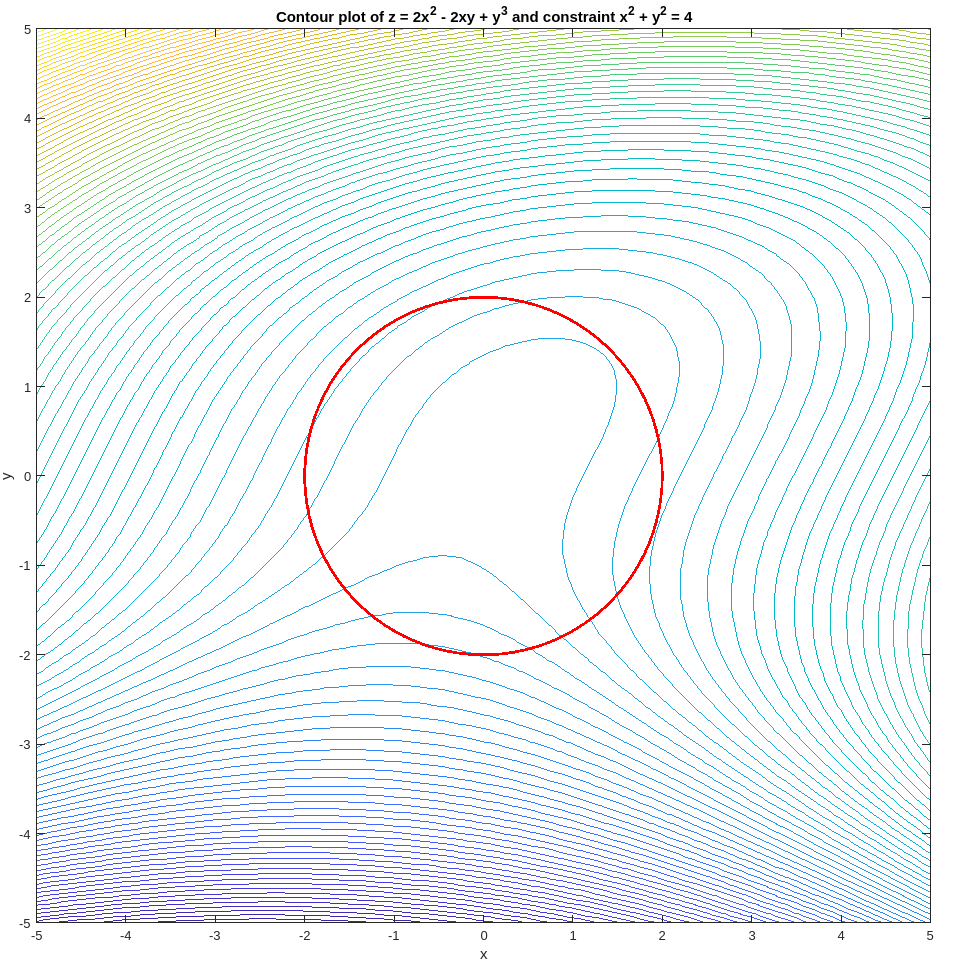
\includegraphics[width=12cm]{graphics/2b.png}
  \caption{The contour plot of the function $z = 2x^2 - 2xy + y^3$ and the constraint $x^2 + y^2 = 4$.}
\end{figure}

\vspace*{1cm}

Code explanation:
\begin{itemize}
  \item \texttt{\color{mygreen}theta = linspace(0, 2*pi, 100)} - create a 1x100 row vector $\theta$ of equally spaced values between 0 and 2$\pi$ radians with 100 elements.
  \item \texttt{\color{mygreen}x\_circle = r*cos(theta)} - compute the x-coordinates of the circle using the $\cos$ function and $\theta$.
  \item \texttt{\color{mygreen}y\_circle = r*sin(theta)} - compute the y-coordinates of the circle using the $\sin$ function and $\theta$.
\end{itemize}

\vspace*{2cm}